\documentclass{tktltiki}
\usepackage{url}
\begin{document}
\title{Keskitetty tunnistautuminen Ruby on Rails -ohjelmistokehyksessä}
\author{Olli Jokinen}
\date{\today}
\level{Pro gradu -tutkielma}
\maketitle
\doublespacing
\faculty{Matemaattis-luonnontieteellinen}
\department{Tietojenkäsittelytieteen laitos}
\subject{Tietojenkäsittelytiede}
\depositeplace{Tietojenkäsittelytieteen laitoksen kirjasto}
\additionalinformation{}
\numberofpagesinformation{\numberofpages\ sivua +
\numberofappendixpages[100] liitesivua}
\classification{A.1 [Introductory and Survey] \\
I.7.m [Document and Text Processing]: Miscellaneous}
\keywords{avainsana}
\begin{abstract}
Tutkielmassa selvitetään keskitetyn tunnistautumispalvelun toteuttamista palvelusuuntautuneiden arkkitehtuurien mukaisissa web-sovellusympäristöissä. Pääpainopisteenä on sovellusympäristöt, joissa ollaan siirtymässä palvelusuuntautuneisiin arkkitehtuureihin. Tutkielmassa käytetään esimerkkinä tällaisesta ympäristöstä Kapsi Internet-käyttäjät ry:n jäsenhallintatyökaluja, joiden tunnistautuminen muutetaan keskitetyn tunnistautumispalvelun tehtäväksi.

Web-sovellusten kehitys ensimmäisistä CGI-ohjelmista kohti palvelusuuntautuneita arkkitehtuureita ja tunnistautumisen tarpeet tällaisissa arkkitehtuureissa esitellään. Tutkielmassa käydään läpi turvallisuuden osatekijöitä ja tavallisia tunnistautumiseen liittyviä ongelmia web-sovelluksissa. Hahmotellaan keskitetty tunnistautumispalvelu ratkaisemaan ongelmia sekä pohditaan sen etuja ja haittoja nykyään käytettyihin tunnistautumismekanismeihin nähden.

Tunnistautumispalvelun ja web-sovelluksen väliseen rajapintaan käytettäviä protokollia (SAML, OpenID ja OAuth) tutkitaan ja esitellään OAuth-protokollaa käyttävä arkkitehtuuri Kapsin järjestelmään. Esitetyn arkkitehtuurin etuja ja haittoja sekä sen soveltamista muihin vastaaviin ympäristöihin tutkitaan. Arkkitehtuurin laajentamista keskitettyyn pääsynvalvontaan ja kertakirjautumiseen pohditaan. Ulkoisen tunnistautumispalvelun käyttöä pohditaan, esimerkkinä Facebookin tarjoama tunnistautumisrajapinta.
\end{abstract}
\mytableofcontents
\section{Johdanto}
Miten käyttäjädataa onko käsitelty ja käsitellään. Kehitys paikallisesti käytetyistä tiedostopohjaisista systeemeistä kohti tietokantoja ja asiaan räätälöihin palveluihin (LDAP). LDAP oleelisin, mutta tutkimuksen kannalta abstraktointi on tärkeä juttu.

Johdanto puoli sivua, alaluvut 0.5-1 sivu.
\section{Ongelmakenttä}
\section{Teknologiat}
\subsection{LDAP}
\subsection{OAuth}
OAuthin kehitystyö alkoi marraskuussa 2006, kun Twitter-pal\-ve\-luun toteutettiin \mbox{OpenID-tukea}. Pian huomattiin, ettei OpenID sovellu käytettäväksi palvelun API-ra\-ja\-pin\-to\-jen kanssa, vaan tarvittiin erillinen pääsynvalvontaprotokolla \cite{oauth_primer}. Siihen asti Twitter-integraatio oli toteutettu pyytämällä käyttäjää antamaan Twitter-tun\-nuk\-sen\-sa ja -salasanansa, joiden avulla palvelu integroitui käyttäjän Twitter-tiliin. Twitterin kehittämä xAuth ja siitä kehittynyt OAuth-protokolla mahdollistavat resurssien käytön ilman käyttäjätunnuksen ja salasanan luovuttamista kolmannelle osapuolelle \cite{oauth2_0}.

OAuthin ensimmäinen versio (1.0) julkaistiin lokakuussa 2007 ja päivitetty versio (1.0a) kesäkuussa 2009 \cite{oauth2_0}. OAuthin versio 2.0 on myös kehitteillä ja se on tarkoitus julkaista marraskuussa 2012 \cite{oauth2_0}. OAuth on määritelty RFC-dokumentissa numero 5849. OAuthin 2.0-version kehitys on ollut vaikeuksissa lähinnä sen jatkuvasti kasvaneiden ominaisuusvaatimusten takia. OAuth 2.0 on kuitenkin käytössä useissa palveluissa, kuten Facebookissa ja GitHubissa, koska OAuth 1.0a:n ominaisuudet eivät ole riittäneet niille. 2.0 helpottaa mm. API-kutsujen tekemistä, koska valtuutusavainten allekirjoitusta on yksinkertaistettu \cite{oauth2_0}.

OAuth on avoin pääsynvalvontaprotokolla hajautetuille web-sovelluksille. Se mahdollistaa käyttäjien resurssien jakamisen palveluiden välillä ilman käyttäjätunnuksen tai salasanan luovuttamista kolmansille osapuolille. Se perustuu erilaisten valtuutusavainten välittämiseen palveluiden kesken \cite{oauth2_0}. Valtuutusavain on allekirjoitettu identiteetintarjoajalla, johon sekä käyttäjä että palvelun toteuttaja luottaa. Muun muassa Facebook tarjoaa avoimen OAuth-rajapinnan, jota web-sovellusten toteuttajat voivat käyttää pääsynvalvonnassaan.

Kuvassa \ref{oauth} on esitetty, kuinka OAuthia käytetään käyttäjän tunnistamiseen. Tunnistautumispalvelin ja käyttäjähallinta voidaan toteuttaa erillisinä palveluina. Tällöin tunnistautumispalvelun antaa pääsyvaltuuden web-sovellukselle, jonka avulla tiedot haetaan käyttäjähallinnasta (kohdat 10 ja 11). Selkeyden vuoksi tunnistautumispalvelun oletetaan toimivan myös käyttäjätietojen jakelijana.

\begin{figure}[!b]
\centering
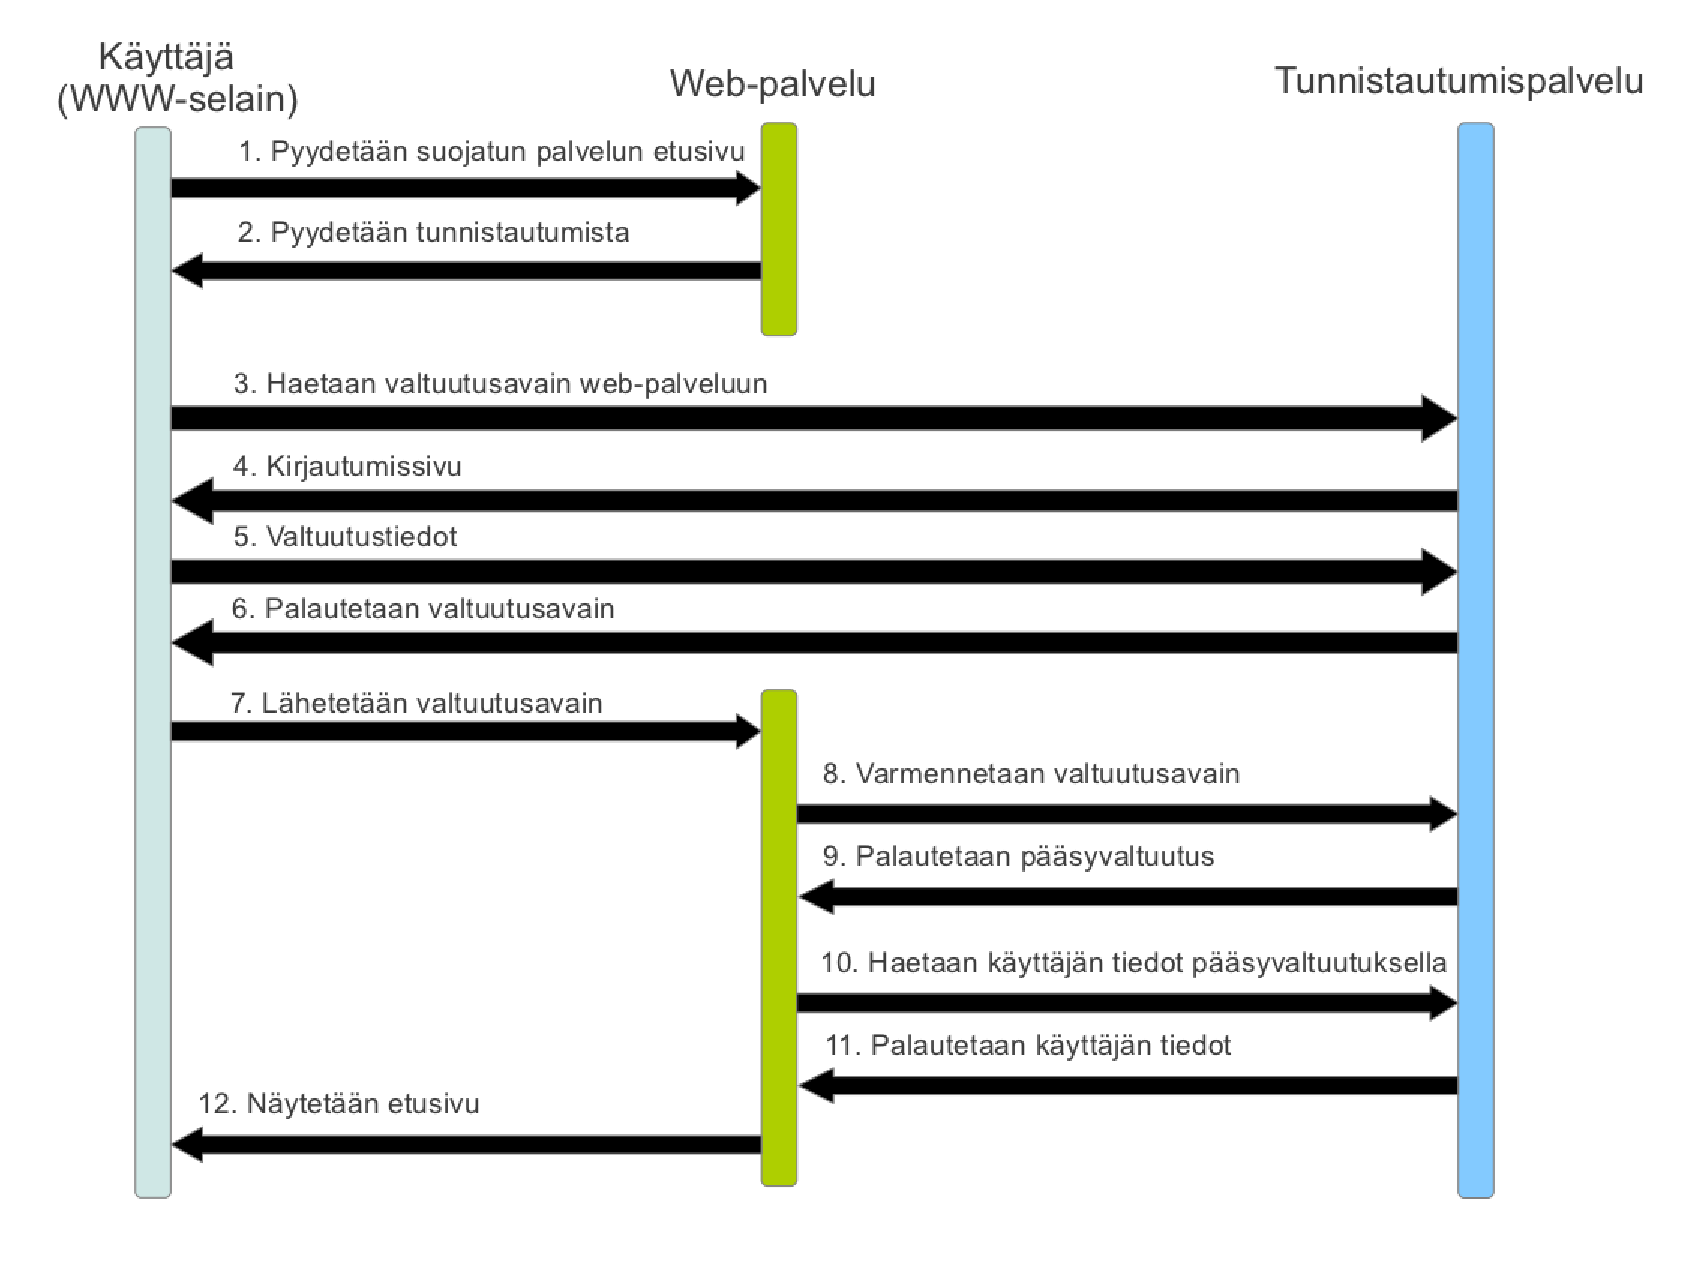
\includegraphics[width=\textwidth]{teknologiat/protokollat/oauth.eps}
\caption{OAuthin toiminta sekvenssikaaviona.}%
\label{oauth}
\end{figure}

OAuthissa valtuutusavaimelle voidaan asettaa erilaisia rajoituksia esimerkiksi sen suhteen, mitä tietoja käyttäjästä annetaan web-sovellukselle tai mihin resursseihin kyseisellä avaimella pääsee käsiksi. Kuvassa \ref{facebook_login} kirjautumisen yhteydessä Porkkanamafialle annetaan oikeus nähdä käyttäjän nimi, profiilikuva, sukupuoli jne. OAuth ei siis ole varsinaisesti tunnistautumisprotokolla, mutta valtuutusavaimen perusteella käyttäjä voidaan yksilöidä: kun käyttäjä kirjautuu myöhemmin uudestaan Porkkanamafiaan, hän hakee valtuutusavaimen Facebookilta, jota käyttämällä Porkkanamafia hakee Facebookista käyttäjän tiedot. Käyttäjän tiedoissa mukana olevalla Facebookin yksilöivällä tunnistenumerolla käyttäjä voidaan todeta samaksi kuin edellisellä kirjautumiskerralla.
\section{Toteutus}
\section{Toteutuksen evaluaatio}
\section{Yhteenveto}
\bibliographystyle{tktl}
\bibliography{munBibTeXtiedosto}
\lastpage
\appendices
\internalappendix{\theappendix}{Eka liite}
Liitetekstiä.
\internalappendix{2}{Toka liite}
Liitetekstiä. Ehkä kuviakin.
\externalappendix{\theappendix}{Ohjelmalistaus joka ei sisälly
\LaTeX-tiedostoon}
\end{document}
